\chapter{Construction of a miniature epi-fluorescence microscope \label{chap-scope}}

\section{Introduction}\todo{edit microscope intro}

One of the major technological limitation in neuroscience research is recording neural activity in model animals. Traditional techniques such multi-unit recordings give excellent temporal resolution, however the spatial resolution --- as measured by the number of cells simutaneously recorded --- is limited. Moreover, it is very hard to distinguish cell subpopulations within the same region from the recording. Neural activity can also be inferred by \textit{post mortem} staining of neural activity markers, such as cfos or arc. This method give excellent spatial resolution, however the temporal resolution is very poor, where the time window of neural activity lasts from minutes to hours.

    Live calcium imaging gives the best of both methods. By labelling the cell of interest with a calcium indicator, neural activity can be recorded in milli-second resolution. Hundreds of cells can be simultaneously recorded, and specific subpopulations can be distinguished by fluorescence in different colour channels. However, traditional live calcium imaging requires the animals' head firmly fixed under a microscope stage. This requirement is incompatible with most well established behaviour assays, and at the same time introduce significant stress to the animal, potentially confounding the behavioural result. Moreover, due to light scattering in the opaque brain tissue, most of the studies have focused only on cortical areas, while techniques to image deep brain tissue on a standard two-photon microscope is still under development and not widely adopted \citep{barretto12}.

    \textit{In vivo} calcium imaging in behaving animals is first demonstrated by Mark Schnitzer's group in Stanford \citep{ghosh11}. The authors constructed a miniature epifluorescence microscope which is chronically implanted in the brain to image the fluorescence from region of interest. In a follow-up paper \citep{ziv13}, the authors demonstrated that the miniature microscope can image GCaMP3 calcium signals from hippocampal \gls{ca1} place cells for more than a month. However, there has been several limitations of their design: first their design incorporates an objective lens of \SI{1}{\mm}  in diameter, which is impractical to reach deep brain tissue; second, their mini-microscope was only able to identify GCaMP signals, and therefore unable to distinguish different cells types within the population \citep{ghosh11,ziv13}. 

    In the current project, we aim to tackle the above mentioned limitations by building a head-mount miniature microscope which is able to image calcium signals in deep brain structures, while also able to image a separate fluorescence colour channel, allowing to distinguish difference cell type. The mini-microscope, once developed, will be used for imaging \gls{la} neurons to investigate mechanisms of fear memory encoding. Moreover, we aim to create an simple open design with little requirement of engineering experience to assemble, so it can be assembled and used cost-efficiently in most neuroscience laboratories. 

\section{Material and Methods}

\subsection{General design of the mini-microscope}

The mini-microscope has the same design as an general single-photon epifluorescence microscope except for the size constraints. Excitation light is emitted from a high-intensity \gls{led} light source, filtered, and reflected by a dichroic mirror to illuminate on the sample. The fluorescent emission light from the sample is collected by the objective, passes through the dichroic mirror, filtered and focused on the camera. To fit the size constraints, we chose the use a high-intensity \gls{led} as the light source, a \gls{grin} lens as an objective, and a miniaturized \gls{cmos} camera to capture the image.\todo{maybe a illustration}

The optical design of the microscope is aided with Zemax software (Zemax Development Corporation) to optimize the lens and filter configuration. The casing of the microscope is modelled using OpenSCAD software. 

\subsubsection{Lens configuration}

The lenses configuration consists of a \gls{grin} objective lens and a ocular barrel lens forming a ``4F system'', where the distance between the thin-lens equivalent of the two lenses equals to the sum of the focal length. Potential lenses for emission light path were selected from modelling and calculation to give a working distance of \SI{100}{\um} in water, a magnification of 6x and a back focal length of \SI{6}{\cm}. During prototyping, the lenses were purchased and installed into custom-made mounts on a two-arm stereotaxic frame. The distance of the lenses are then optimized against a fibre bundle light source close to the \gls{grin} lens. A drum lens is used to collect light from the \gls{led}. The drum lens is tested in a similar manner and selected to give diverging light after \gls{grin} lens. We has chose to use an achromatic doublet (F=\SI{15}{\mm}, Edmund Optics). We used a \SI{1.8}{\mm} diameter 0.25-pitch \gls{grin} lens (64--537, Edmund Optics) as objective for hippocampus imaging. To minimize brain damage for deep brain imaging, the objective lens was a home-assembled doublet of a \SI{0.5}{\mm} diameter, 1-pitch \gls{grin} relay lens (ILW-050-P050, GoFoton) and a \SI{2}{\mm} diameter 0.25-pitch \gls{grin} lens (ILW-200-P025, GoFoton). The details of doublet assembly is described in \label{objective assmebly}.

\subsubsection{Filter selection}
The filters were selected to cover the excitation and emission spectrum of the genetic encoded calcium sensor GCaMP6f \citep{chen13} and further screened for high bandwidth and low overlap. To fit the size constraints, the excitation and emission filters had dimensions of \SI{5x5x1}{\mm}, and the dichroic mirror \SI{7.1x5x1}{\mm}. We chose to use a \gls{fitc} filter set for gCaMP6 imaging (49002, Chroma). For dual colour imaging, we took advantage of broad excitation spectrum of the red retrobeads, and use the same blue light to excite the red fluorophore. In these experiments, a \acrshort{tritc}\slash\acrshort{fitc} with single band exciter filter set was used (59204, Chroma).

\subsubsection{Electronics}
The image sensor are selected to have an packaged size of less than \SI{1.5 x 1.5}{\cm}. We used a commercially available analogue camera module (HD1313BW, Ruishibao) that gives satisfactory sensitivity and dynamic range. The camera board is connected to a \SI{5}{\V} power regulator. After the power regulator, the wires were connected through a slip ring (SRC012-C, Adafruit) was the used to avoid entanglement of the wires during animal behaviour. After the slip ring, the wires are connected to a \SI{12}{\V} \gls{dc} power source and a \gls{usb} analogue video capture card (Capit, Mygica). The video capture card is controlled by custom software for synchronized video capture.  Alternatively, a board-level miniature integrated digital camera (MU9PM-MBRD, XIMEA) can be used. While the XIMEA camera adds significant cost to the miniature microscope, it however allows custom control of camera parameters such as pixel binning, gain and exposure. The XIMEA also output in 12-bit per pixel, and gives better overall \gls{snr}.

A monochrome, high-intensity blue \gls{led} (LXML-PB01-0023, Lumiled) was used as the light source. The \gls{led} wires joins the video camera wires through the slip ring, and then connected to a variable \gls{dc} power source. During recording, the \gls{led} was driven at a current between \SI{20}{\mA} and \SI{50}{\mA}.

\subsubsection{Casing and assembly}
The casing was printed in black resin using a Form 2 3D printer (Formlabs). This gives a rigid, opaque and black casing with highest resolution for details. The microscope body is screwed onto the camera holder via M8 thread to allow easy change of the focus plane. A side M2$\times$\SI{2}{\mm} nylon screw is used to lock the camera holder on the microscope body and fix the focus of the mini-microscope.

A metal nut \todo{microscope body nut spec} was glued to the bottom of the microscopy body concentric to the light path opening using a fast-curing epoxy glue (\todo{epoxy info?}). The nut allows to easily and firmly lock the microscope onto the baseplate.

Unlike the microscope body, the base plate was 3d printed using \gls{fdm} with \gls{pla} material. A threaded tube (\todo{baseplate thread tube info}) was heated with a soldering iron and inserted into the center of the base plate, and further fixed with epoxy glue. The objective lens was inserted into the center of the threaded tube, and fixed with crazy glue on the bottom. For objective that are thinner than the inner diameter of the threaded tube, an additional stainless steel tube was inserted inbetween to aid alignment of the lens.

\subsubsection{Objective lens assembly for deep brain imaging} \label{objective assembly}

For deep brain imaging, a \SI{0.5}{\mm} diameter, 1.0-pitch relay lens was glued to a \SI{2}{\mm} diameter, 0.25-pitch \gls{grin} lens. The setup is modified from \citep{kim12} to ensure concentricity and alignment. In the setup, a V-groove clamp (\todo{clamp details}, ThorLab) is used to hold the large \gls{grin} lens in place virtically, and the thin relay lens was mounted on another V-groove clamp attached to a 3-axis manipulator (\todo{manipulator details}, ThorLabs). The two V-groove clamps were leveled using a bull's eye spirit level. An analogue lens and camera chip was mounted under the large \gls{grin} lens, and displayed the image of the large \gls{grin} lens on a monitor. A disecting microscope was mounted horizontally for monitoring the vertical position of the two lenses. \todo{insert figure for the setup}

During assembly, both lenses were mounted in the V-groove clamps respectively. A small drop of \gls{uv} curing optical adhesive (NOA61, Norland) was added to the bottom surface of the relay lens using a 27-gauge needle. The relay lens was then lower to just above the large \gls{grin} lens when an image of the relay lens is visible on the monitor. The relay lens was then moved to the center of the large \gls{grin} lens according to the monitor display. Observed through the dissecting microscope, the relay lens was then lowered to touch the upper surface of the large \gls{grin} lens. A \SI{375}{\nm} spot \gls{uv} light source (\todo{uv light source info}) was used to cure the optical glue. The curing time is calculated to give at least \SI{3}{\J\per\mm\squared} of \gls{uv} light on the optical adhesive. 


\subsection{Implantation of the mini-microscope}

Two weeks after gCaMP6 infusion to the target area, animals are anesthesized and head-fixed on a stereotaxic frame as described in \todo{ref general methods}. Three screws were placed around the viral injection site for anchoring the microscope. 

For implantation targetting \gls{ca1}, a circular craniology of \SI{2}{\mm} was performed above the viral injection site. The dura was pierced and lifted with a fine tweezer to expose the brain. The brain is then constantly irrigated with artificial cerebral-spinal cord fluid to remove the blood. A 27-gauge aspiration needle was used to remove cortex and expose \gls{ca1}. For implantation targetting amygdala after anchoring the screws, a 27-gauge needle was lowered to the target coordinate, left for \SI{5}{\min}, and slowly retracted.

The mini-microscope is then fixed on the stereotaxic frame and gradually lowered to the target coordinates (\gls{ca1}: \gls{la}: \todo{coordinate for ca1 and amygdala}). Opaque black dental acrylic was used to secure the microscope baseplate to the skull. Once the dental acrylic cured, the microscope body was detached from the baseplate and replaced with a cap. Animals were given \SI{5}{\mg\per\kg} ketoprofen for analgesia.

\subsection{In vivo mini-microscope testing}
After lens implantation, the animals were kept in the home cage for at least two weeks before the first image session. This time allows the optical window to clear up. The animals were scruffed, the cap was removed and replaced with the microscope body. A typical imaging session lasts for \SI{5}{\minute}. After the imaging session the microscope body was removed, and the animal was recapped.

\subsection{Image analysis}
\subsubsection{Illumination correction}
\todo{illumination correction meth}
\subsubsection{Motion correction}
\todo{motion correction meth}

\subsubsection{Extracting cell from calcium imaging video}
Individual cell calcium signals were extracted from the movie as previously described \citep{mukamel09}. Briefly, we first estimate the number of cells in the movie, and reduced the number of temporal dimension to roughly number of cells using principle component analysis. The resulting principle components were then subjected to independent component analysis, where the spatial filter for individual cells were extracted from the components, and the calcium signal of the corresponding cell was extracted from the mixing matrix. The time-course calcium signal was then aligned with behaviour recordings to identify neural activity patterns.

\subsubsection{Mapping cells across session}
Cells are extracted from the recordings for both session respectively. The position of the each cells were calculated as the center of mass of the 90 percent pixels in the extracted \gls{ica} component. The position of cells for each recording were approximately aligned to have overlapping center of mass, then rotated to have overlapping principle component vectors. The two point clouds are then precisely aligned using TrimICP(\todo{ref TrimICP}). TrimICP is robust against outliers, which can be observed even when cells fire in one session but were silent in another. TrimICP was performed using a 40\% outlier ratio, optimizing both translation and rotation. After alignment, cells that are less than \SI{5}{\um} from one session to another are mark as  same cells.


\section{Results}

\subsection{mini-microscope}
The mini-microscope provides a cheap and easy way for neuroscience laboratories to measure calcium activity in freely behaving small animals. The completely assembled mini-microscope weighs less than \SI{3}{\g}, and can be bounded in a \SI{25 x 16 x 11}{\mm} box (Figure~\ref{f.scope}). Adult mice with the mini-microscope attached are able to rear, groom, and freely explore environment with no noticable change from their natural behaviour (\todo{mouse image?}).

\todo{insert microscope photo and mouse figure here}
\begin{figure}[h]
    \begin{subfigure}[t]{.5\textwidth}
        \centering
        \includegraphics[width=\textwidth]{scope-cropped}
        \caption{\label{f.scope}}
    \end{subfigure}
    \begin{subfigure}[t]{.5\textwidth}
        \centering
        \missingfigure{animal with scope}
    \end{subfigure}
\end{figure}

The theoretical optical resolution of the mini-microscope is \SI{1}{\um}. To measure the resolution empirically, we tested the mini-microscope against \gls{usaf} resolution target (\todo{USAF target detail}, Edmund Optics). As shown in Figure~\ref{f.usaf}, the thinest lines (group 7 element 6, \SI{2.07}{\um} width) are clearly visible. This suggest that the empirical resolution of the microscope is smaller than \SI{2}{\um}. With this resolution, the mini-microscope is able to resolve cell bodies and capillary blood vessels.

In order to test the illumination, we expressed \gls{gfp} in \gls{la} of an animal, perfused and harvested the brain 3 days later when the \gls{hsv} expression peaks. The brain was sliced coronally on a vibratome until the area of infection. The trunk of the brain was imaged under the mini-microscope. As seen is Figure~\ref{f.scope-gfp}, the \gls{gfp} cells are clearly visible. Moreover, many of the apical dendrites can also be resolved. The imaging quality is comparable to that taken under a standard epi-flourescence microscope (Nikon \todo{Nikon details}\todo{insert Nikon image}. The imaging quality is lower than normal due to the thickness of the brain trunk). This result confirms that the flourescence under the \gls{led} illumination can be reliably detected by the \gls{cmos} camera.

\todo{reorganize figures}
\begin{figure}[h]
    \begin{subfigure}[t]{.55\textwidth}
        \centering
        \includegraphics[width=\textwidth]{microscope-schematic.png}
        \caption{\label{f.scope-schema}}
    \end{subfigure}
    \begin{subfigure}[t]{.45\textwidth}
        \centering
        \includegraphics[width=\textwidth]{scope-cropped}
        \caption{\label{f.scope}}
    \end{subfigure}
    \begin{subfigure}[t]{.5\textwidth}
        \centering
        \includegraphics[width=\textwidth]{usaf-target.png}
        \caption{\label{f.usaf}}
    \end{subfigure}
    \begin{subfigure}[t]{.5\textwidth}
        \centering
        \includegraphics[width=\textwidth]{scope-gfp.png}
        \caption{\label{f.scope-gfp}}
    \end{subfigure}
    \caption{\subref{f.scope-schema} Schematic of the miniature microscope. Excitation light is emitted from a high-intensity blue LED, filtered and reflected to the sample by a dichroic mirror. GCaMP6 emission is collected by the gradient-index (GRIN) lens, filtered and focused onto a CMOS camera chip, where the images are sent to a computer and recorded. 
             \subref{f.scope} Prototype of the mini-microscope.
             \subref{f.usaf} USAF resolution test target under the mini-microscope.}
             \subref{f.scope-gfp} GFP-expressing cells in perfused brain under the miniature microscope.
\end{figure}

\subsection{Video preprocessing}
\subsubsection{illumination correction}
\todo{move to methods?}
Due to the size limitation of the mini-microscope, the illumination has to be compromized and is uneven. The uneven illumination not only affects the calcium signal and cell detection, but also adds difficulty to the motion correction step, since the uneven illumination pattern appears stable even when there is relative movement between the mini-microscope and the target. To correct this, a 2D gaussian filter with large window (15 $\times$ 15) is convolved with each frame to extract the illumination pattern. The illumination pattern is then subtracted from the frame\todo{... and nomalized by multiplying the inverse of the difference of illumination pattern to roof}. Figure~\ref{f.illumination}\todo{image} shows the maximum projection of the recording before and after illumination correction. Cells under intense illumination in the center can be clearly visualized after illumination correction.

\begin{figure}[h]
    \begin{subfigure}[t]{.5\textwidth}
        \centering
        \missingfigure{before correction}
    \end{subfigure}
    \begin{subfigure}[t]{.5\textwidth}
        \centering
        \missingfigure{after correction}
    \end{subfigure}
    \caption{\label{f.illumination}, before, after}
\end{figure}

\subsubsection{motion correction}
After illumination correction, the movie was then removed from dust, and corrected for motion. Occasional dust speckles on the camera appears as stational small dark objects in the movie, and would interfere with motion detection. To remove the dust speckles, for each frame, pixels two standard deviation darker than mean intensity are labeled. The labeled pixels are morphologically eroded and dilated to remove noise, and then inpainted using Navier-Stokes based methods (\todo{reference opencv?}).

As the motion is almost entirely translational, after dust removal we used phase correlation algorithm to achieved sub-pixel level motion correction. The reference frame is initialized to be the first frame. A moving average of 25 registered frames were generated, and the reference frame is updated by maximum projection of the moving average frame to the reference frame. To test the efficacy of the motion correction algorithm, we have generated a perticularly shaky recording by loosing the connection of the mini-microscope to the baseplate. As can be seen from the maximum projection of the original recording and stabilized recording (Figure~\todo{ref max projection image}), the motion correction works well even for extremely erratic motion. 

\missingfigure{max projection, x/y motion plot}

\subsection{Measuring blood flow with mini-microscope}
To test \textit{in vivo} imaging capability of the microscope, we first implanted the microscope above the cortex, and injected \SI{150}{\ul} of fluorescein-dextran (molecular weight \SI{120}{\kilo\dalton}). The fluorescein-dextran will fill the blood vessels and have similar excitation and emission wavelength to GCaMP. As expected, after fluorescein-dextran injection, the blood vessels are clearly visible when the microscope is implanted (Figure~\ref{f.bloodvessel}).
\todo{calculating blood flow}
\todo{image, blood vessel detection, velocity heatmap}
\begin{figure}[h]
    \includegraphics[width=\textwidth]{blood-vessel.png}
    \caption{\textit{In vivo} image of blood vessel. The animal received 10mg/kg fluorescein-dextran in tail vein. The mini-microscope is placed at cortex when the animal is under anaesthesia. \label{f.bloodvessel}}
\end{figure}


\subsection{Recording calcium transients in CA1}
To test GCaMP6s expression \textit{in vivo}, we infused AAV--syn--GCaMP6s--WPRE into \gls{ca1} hippocampus and implanted the mini-microscope above the injection site. During behavioural session, the animal was placed in a novel environment to explore for \SI{5}{\minute}, during which GCaMP6 fluorescence were recorded. The maximum projection of the GCaMP6 fluorescence in a 5-minute session is shown in Figure~\ref{f.ca1bw}. We were able to extract 200 cells from the recording and their corresponding \ce{Ca^2+} transients (Figure~\ref{f.ca1rainbow}\ref{f.analysis}).

The positions of the animal was traced out in the behaviour video. The timecourse of the identified cells were mapped back to the behaviour of the animal. Figure~\ref{f.traceplot} shows \ce{Ca^2+} activity of potential place cells as they respond to specific location in the environment the animal is in.
\todo{max projection, sample cell, animal tracing, place cell heat map}
\begin{figure}[h]
    \includegraphics[width=\textwidth]{cells-bw.png}
    \caption{Cells in CA1 captured by the mini-microscope in behaving animal. Two weeks after AAV infusion and microscope implantation, the animal is allowed to freely explore a novel environment. The picture is a maximum projection of all frames captured in a 5-minute session. \label{f.ca1bw}}
\end{figure}

\begin{figure}[h]
    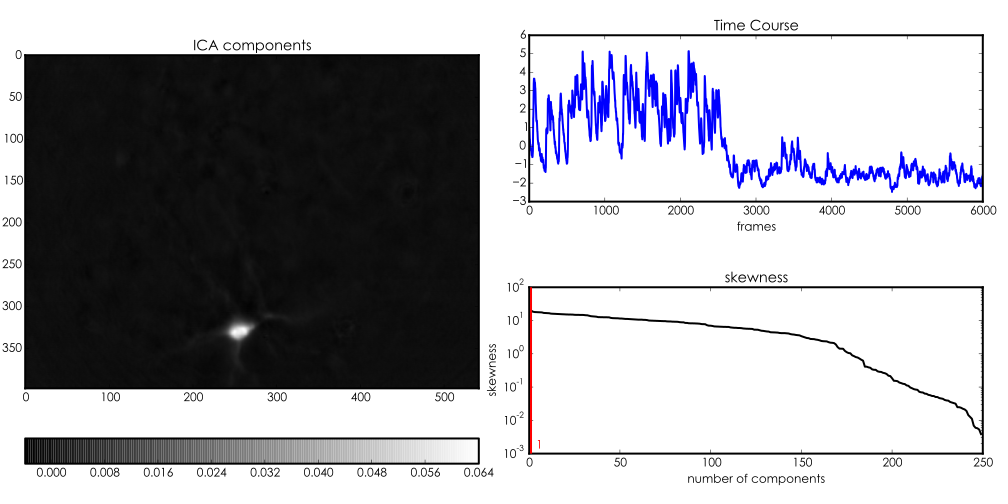
\includegraphics[width=\textwidth]{analysis1.png}
    \caption{Example of an independent component of the movie after analysis, showing both the extracted spatial location of the cell (left) and the un-normalized actvity (top right). \label{f.analysis}}
\end{figure}


\begin{figure}[h]
    \includegraphics[width=\textwidth]{cells-bw-rainbow-all-final.png}
    \caption{More than 100 cells are identified in a single imaging session. The identified cells are randomly coloured. \label{f.ca1rainbow}}
\end{figure}


\begin{figure}[h]
    \begin{subfigure}[t]{.5\linewidth}
        \includegraphics[width=\textwidth]{trace1.png}
    \end{subfigure}
    \begin{subfigure}[t]{.5\linewidth}
        \includegraphics[width=\textwidth]{trace2.png}
    \end{subfigure}
    \begin{subfigure}[t]{.5\linewidth}
        \includegraphics[width=\textwidth]{trace3.png}
    \end{subfigure}
    \begin{subfigure}[t]{.5\linewidth}
        \includegraphics[width=\textwidth]{trace4.png}
    \end{subfigure}
    \caption{Activity of 4 sample cells plotted against location of the animal. The colour represents the \ce{Ca^2+} activity. The cellular activity is specific to the animal's location in the environment. \label{f.traceplot}}
\end{figure}

\subsection{between session stability}
Two measure the stability of the imaging field between sessions, animals with gCaMP6 infused in \gls{ca1} underwent contextual fear conditioning, and \SI{24}{\hour} later, were put back to the same context for testing. Mini-microscope was attached during both imaging sessions, and the recordings are aligned as shown in \todo{alignment figure}. \todo{alignment result, how many percentage overlap??}
\todo{figure matching cells across sessions}

\subsection{Deep brain imaging}
\begin{figure}[h]
    \centering
    \includegraphics[width=\textwidth]{amygdala.png}
    \caption{Raw calcium signals during fear conditioning. Left: extracted map of neurons, randomly coloured. Right: Sample calcium signals over time.\label{f.amygdala}}

\end{figure}
\todo{same as CA1 analysis}
This design of the miniature microscope incorporates an objective lens of \SI{1.8}{\mm} in diameter. This lens is both too thick and too short to reach deep brain structures such as amygdala. We have modified the design and attached a \SI{4.8}{\mm} long \SI{0.5}{\mm} diameter relay \gls{grin} lens (ILW-050-P050, GoFoton) to the objective lens. Attaching the relay lens does not significantly alter the imaging ability of the microscope, however allows the lens to reach deep brain regions without extensive damage. With this configuration, we are able to visualize activity form more than 40 cells in lateral amygdala and track them over time (Figure~\ref{f.amygdala}).


\subsection{Two colour}
To test the two-colour version of the mini-microscope, we infused red retrobeads (\todo{retrobeads info}) in \gls{nac} bilaterally and gCaMP6 \gls{aav} in \gls{la}. The retrobeads will be trafficked retrogradely along axons, and will label \gls{la} neurons that preject to \gls{nac}. The images acquired from both the green and red channel are shown in Figure~\ref{f.twocolour.g.invivo},\ref{f.twocolour.r.invivo}. There is no interference between the two channels\todo{wording}.

\begin{figure}[h]
    \begin{subfigure}[t]{.5\linewidth}
        \includegraphics[width=\textwidth]{two-colour-g.png}
        \caption{\label{f.twocolour.g}}
    \end{subfigure}
    \begin{subfigure}[t]{.5\linewidth}
        \includegraphics[width=\textwidth]{two-colour-r.png}
        \caption{\label{f.twocolour.r}}
    \end{subfigure}
    \begin{subfigure}[t]{.5\linewidth}
        \includegraphics[width=\textwidth]{two-colour-green-in-vivo.png}
        \caption{\label{f.twocolour.g.invivo}}
    \end{subfigure}
    \begin{subfigure}[t]{.5\linewidth}
        \includegraphics[width=\textwidth]{two-colour-red-in-vivo.png}
        \caption{\label{f.twocolour.r.invivo}}
    \end{subfigure}

    \caption{Images of cells with different fluorescent protein under the two-colour mini-microscope prototype. \subref{f.twocolour.g} HSV-GFP in perfused brain. \subref{f.twocolour.r} HSV-tdTomato in perfused brain. \subref{f.twocolour.g.invivo} Red retrobeads \textit{in vivo} in green channel. \subref{f.twocolour.r.invivo} Red retrobeads \textit{in vivo} in red channel. \label{f.twocolour}}
\end{figure}

















\begin{comment}
\begin{figure}[h]
    \includegraphics[width=\textwidth]{behaviour-schematic.png}
    \caption{Proposed experiment. A mixture of GCaMP6s-expressing AAV and tdTomato-expressing long-term HSV are infused into LA of the animals. A two-colour microscope is implanted to visualize infected LA neurons. The animal then subject to auditory fear conditioning paradigm, and GCaMP6s signals in either tdTomato\textsuperscript{+} or tdTomato\textsuperscript{-} cells are recorded. We hypothesize that the tdTomato\textsuperscript{+} cells will be more excitable than tdTomato\textsuperscript{-} cells during training and testing. \label{f.behaviour-schema}}
\end{figure}
\end{comment}




\section{Discussion}

In the current project, we have developed a miniature microscope that allows deep brain calcium imaging in freely behaving mice. The mini-microscope weighs less than \SI{3}{\gram}, and can be implanted on a mouse's head without altering the mouse's natural behaviour. We have successfully used it to record calcium transients both from \gls{ca1} in dorsal hippocampus and lateral amygdala. Moreover, we have added an additional red colour channel for subpopulation identification. With the additional colour channel, we have shown that it is possible to identify the projection target of the cell using flourescent retrobeads. 

Compared to previous designs of mini-microscope, our design is simpler to build and more cost efficient, and suitable for use for common neuroscience laboratories. All optical and electronic parts are commercially available, and the casing can be 3D-printed. The mini-microscope is designed to be easily assembled with minimal tools. The design allows biology researchers with minimal engineering experience to build the mini-microscope and use it for biological research. Moreover, the complete cost a single mini-microscope is between \$\,300 and \$\,1000, and will not representa significant expense in most biology laboratories.

Here we used PCA--ICA for sorting the cells from videos. It is worth noting that although this method often can extract cells and traces reliably, it is not optimal: the PCA--ICA can only catch statistical regularities in the cell activity, but any spatial information is discarded. As a result of this, if the duration of the video is relative short, or some cells fires in synchrony, the PCA--ICA is unable to extract individual cells well. In addition, the result of PCA--ICA may include negative values in the cell activity, which should be limited to only posititive values. Recently, \citet{pnevmatikakis16} used a \gls{cnmf} approach for cell sorting from calcium imaging videos. This method is superior from PCA--ICA in videos acquired from two-photon microscopes, and is promising to be applied to the mini-microscope dataset. 

In the two-colour version of the mini-microscope, colour aberration still exists, such that the alignment of the red and green channels is not perfect. However, the colour abberation is not significant, and will only result in a theoretical shift of \SI{2}{\um} in the field of view. Given that the diametor of a neuron is usually more than \SI{10}{\um}, this misalignment will not significant affect the identification of neural subpopulations in the red channel. The colour abberation is primarily introduced by the \gls{grin} lens, and can be corrected by a careful selection of the barrel lens. Additionally, the colour abberation can also be corrected by a \gls{grin} lens with optimal radial refractory index profile. However although technically possible, such \gls{grin} lens is not currently commercially available. 




